\documentclass[]{article}

\usepackage[utf8]{inputenc}
\usepackage[english,serbian]{babel}
\usepackage[margin=0.7in]{geometry}
\usepackage{url}
\usepackage{float}
\usepackage[graphicx]{realboxes}
\usepackage{listings}
\usepackage{textcomp}
\usepackage{xcolor}
\usepackage{titlesec}
\usepackage{adjustbox}
\lstset {
    language=HTML,
    frame=none,
    %xleftmargin=-.25in,
    %xrightmargin=.25in
    framesep=10pt,
    tabsize=4,
    showstringspaces=false,
    upquote=true,
    commentstyle=\color{black},
    keywordstyle=\color{black},
    stringstyle=\color{black},
    basicstyle=\small\ttfamily,
    emph={int,char,double,float,unsigned,void,bool},
    emphstyle={\color{black}},
    escapechar=\&,
    classoffset=1,
    morekeywords={>,<,.,;,,,-,!,=,~},
    keywordstyle=\color{black},
    classoffset=0,
    breaklines=true
}
\pagenumbering{gobble}

\titlespacing\title{left spacing}{before spacing}{after spacing}[right]

\title{Ra\v{c}unarske mre\v{z}e 4I, Ispit - Septembar 1}
\date{25.08.2019.}

\begin{document}

\makeatletter
\begin{center}

{\fontsize{12pt}{14pt}\selectfont\bfseries\@title\par}
\@date
\vspace{5mm}

Pro\v{c}itati sve zadatke \textbf{pa\v{z}ljivo} pre rada - sve \v{s}to nije navedeno ne mora da se implementira! 

Na \texttt{Desktop}-u napraviti folder sa imenom u formatu \texttt{rm\_sept1\_Ime\_Prezime\_miGGXXX} i u njega smestiti \texttt{Java} projekat sa resenjima zadataka u zasebnim paketima sa imenima \texttt{zad1}, \texttt{zad2} itd. 

Vreme za rad: \textbf{2.5h}. Sre\'{c}no!
\end{center}
\makeatother


\begin{enumerate}
  \item Sockets \textbf{(15p)}
  \begin{itemize}
    \item Napraviti Java aplikaciju koja ima ulogu pojednostavljenog anonimnog FTP klijenta. Povezati se na lokalni server na portu 12345 koriste\'c{}i \texttt{Socket} klasu. Omogu\'c{}iti da klijent mo\v{z}e poslati serveru liniju pro\v{c}itanu sa standardnog ulaza (u stavkama ispod ova linija \'c{}e predstavljati relativnu putanju do fajla). Implementirati jednostavni \emph{echo} odgovor od strane servera prilikom testiranja klijenta. \hfill (4p)
    \item Napraviti Java aplikaciju koja ima ulogu pojednostavljenog FTP servera. Pokrenuti lokalni server na portu 12345 koriste\'c{}i \texttt{ServerSocket} klasu. Server svim povezanim klijentima prosledjuje sadr\v{z}aj fajla sa relativne putanje koju su prosledili serveru. Prilikom povezivanja na server svaki klijent se obradjuje u zasebnoj niti. Postarati se da se fajlovi baferisano \v{s}alju klijentima. \hfill (5p)
    \item Implementaciju klijenta izmeniti tako da primljene bajtove \v{c}uva u fajl sa imenom uzetim iz unete relativne putanje. \hfill (2p)
    \item Pre slanja fajla klijentu server \v{s}alje indikator uspeha zahteva (jedan bajt). Ukoliko fajl na tra\v{z}enoj putanji postoji i mo\v{z}e se poslati klijentu, indikator ima vrednost $0$. U protivnom, ukoliko fajl ne postoji ili putanja cilja fajl koji se ne nalazi unutar korenog foldera servera, indikator ima vrednost $1$ i konekcija se prekida nakon slanja indikatora. Klijent posle slanja relativne putanje \v{c}eka na indikator a zatim na osnovu pristigle vrednosti ili ispisuje poruku o neuspehu ili nastavlja sa preuzimanjem. \hfill (3p)
    \item Postarati se da su svi resursi ispravno zatvoreni u slu\v{c}aju izuzetka. \hfill (1p)
  \end{itemize}

  \item Swing \textbf{(15p)}
  \begin{itemize}
    \item Napraviti prozor i u njega dodati skrolabilnu komponentu za prikaz sadr\v{z}aja web stranice. \hfill (1p)
    \item Omogu\'c{}iti da je pra\'c{}enje linkova podr\v{z}ano - kada se link aktivira promeniti sadr\v{z}aj komponente za prikaz tako da prikazuje web stranicu na koju link pokazuje (za testiranje napraviti par lokalnih HTML fajlova sa linkovima izmedju njih, primeri su dati na narednoj strani). \hfill (2p)
    \item Dodati dugme \texttt{Undo} (na slici ozna\v{c}eno karakterom \texttt{<}) na \v{c}iji klik se sadr\v{z}aj komponente za prikaz vra\'c{}a na sadr\v{z}aj prethodne web-strane koja je bila prikazana (ukoliko takva postoji). \hfill (2p)
    \item Dodati dugme \texttt{Redo} (na slici ozna\v{c}eno karakterom \texttt{>}) na \v{c}iji klik se sadr\v{z}aj komponente za prikaz vra\'c{}a na sadr\v{z}aj naredne web-strane koja je bila prikazana pre Undo operacije (ukoliko takva postoji). \hfill (2p)
    \item Dodati dugme \texttt{ca} \v{c}iji je efekat da ukloni sve linkove iz komponente za prikaz. Preciznije, na klik ovog dugmeta se HTML sadr\v{z}aj komponente za prikaz \v{c}isti od svih \texttt{a} tagova (zajedno sa njihovim atributima) dok njihov sadr\v{z}aj \textbf{ostaje prisutan}. Tako dobijeni filtrirani HTML prikazati u komponenti za prikaz. \hfill (5p)
    \item Ispo\v{s}tovati izgled aplikacije (ne me\v{s}ati redosled komponenti i postarati se da su odnosi u veli\v{c}ini kao na slici na narednoj strani). \hfill (2p)
    \item Omogu\'c{}iti da se prozor mo\v{z}e pro\v{s}iriti i smanjiti a da se raspored i razmera komponenti ne promeni. \hfill (1p)
  \end{itemize}

\end{enumerate}


\newpage

\begin{figure}[H]
  \centering
  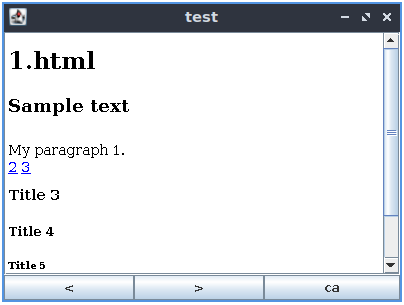
\includegraphics[scale=0.7]{fig1.PNG}
  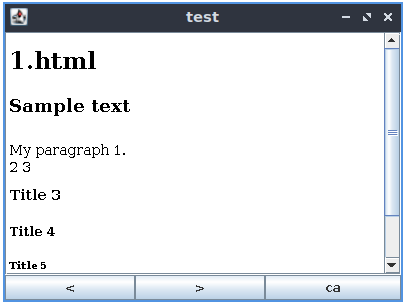
\includegraphics[scale=0.7]{fig2.PNG}
  \label{fig2}
  \caption{Izgled aplikacije pre i posle aktivacije dugmeta \texttt{ca}}
\end{figure}


HTML test fajlovi:\\

\noindent
\begin{tabular}{ccc}
\begin{lstlisting}
  <!DOCTYPE html>
  <html>
    <body>
      <h1>1.html</h1>
      <h2>Sample text</h2>
      
      <p>My paragraph 1.</p>

      <a href="2.html">2</a>
      <a href="3.html">3</a>

      <h3>Title 3</h3>
      <h4>Title 4</h4>
      <h5>Title 5</h5>
      <h6>Title 6</h6>

      Some text goes here.
    </body>
  </html>
\end{lstlisting}&
\begin{lstlisting}
  <!DOCTYPE html>
  <html>
    <body>
      <h1>2.html</h1>
      <h2>Sample text</h2>
      
      <p>My paragraph 2.</p>

      <a href="1.html">1</a>
      <a href="3.html">3</a>

      <h2>Title 2</h2>
      <h1>Title 1</h1>
      <h5>Title 5</h5>
      <h4>Title 4</h4>

      Text text text text.
    </body>
  </html>
\end{lstlisting}&
\begin{lstlisting}
  <!DOCTYPE html>
  <html>
    <body>
      <h1>3.html</h1>
      <h2>Sample text</h2>
      
      <p>My paragraph 3.</p>

      <a href="1.html" 
          id="1">1</a>
      <a href="2.html" 
          class="2">2</a>

      <h4>Title 4</h4>
      <h5>Title 5</h5>
      <h6>Title 6</h6>
      <h2>Title 2</h2>

      Text text text text.
    </body>
  </html>
\end{lstlisting}
\end{tabular} 

\end{document}
